\begin{frame}[fragile]{Segmented Scan}{Implementation}
    \begin{itemize}
     \item Not present in STL!
     \item No reference implementations...
    \end{itemize}
    \vspace{10pt}
    Solution: Wrapping the binary operation!
    
    
    \begin{lstlisting}[language=C++, frame=single, gobble=4]
    [binary_op](PairType left, PairType right){
        PairType new_right = right;
        if (not right.flag)
            new_right.value =
                binary_op(left.value, right.value);
        return new_right;
    });
    \end{lstlisting}
\end{frame} 
% 
% \begin{frame}{Segmented Scan}{Problem with the Wrapper}
%  \centering
%  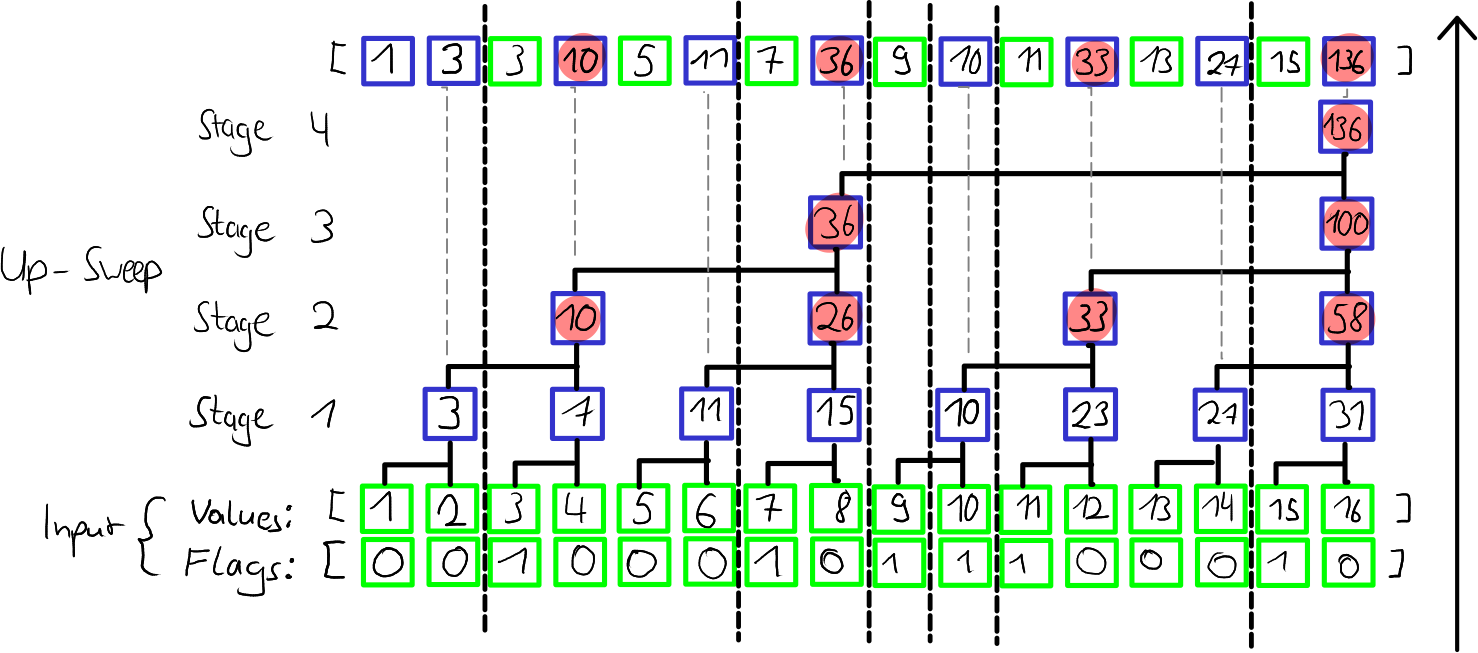
\includegraphics[width=\textwidth]{wiki/ProblemSegmentedUpDown}
% \end{frame}
% 
% \begin{frame}[fragile]{Segmented Scan}{Solution}
%     \begin{lstlisting}[language=C++, frame=single, gobble=4]
%     [binary_op](PairType left, PairType right){
%         PairType new_right = right;
%         if (not right.flag)
%             new_right.value =
%                 binary_op(left.value, right.value);
%             if(left.flag){
%                 new_right.flag = left.flag;
%             }
%         }
%         return new_right;
%     });
%     \end{lstlisting}
% \end{frame}

% \begin{frame}[fragile]{Segmented Scan}{Solution}
%     \begin{lstlisting}[language=C++, frame=single, gobble=4]
%     if(left.flag)
%         new_right.flag = left.flag;
%     \end{lstlisting}
%     \missingfigure{Explanation of operator}
% \end{frame}

\begin{frame}[fragile]{Segmented Scan}{Solution}
\todo{shorter }
Works for:
\begin{itemize}
 \item STL Scans
 \item tbb::parallel\_scan Inclusive
 \item Up-Down Sweeping Scan inclusive
 \item Tiled Scan Inclusive
\end{itemize}
\vspace{10pt}
Challenge: Exclusive Scan
\begin{itemize}
 \item Working Copy of Flags!
 \item Up-Down Sweep!
\end{itemize}
$\Rightarrow$ Exclusive Segmented is complex

\end{frame}


\begin{frame}{Sequential Segmented Scan Results}
 
  \centering
  \vspace{-5pt}
  \includegraphics[width=0.90\textwidth]{"graphs/mp-media Sequential Segmented Scans"}
 
\end{frame}

\begin{frame}{Parallel Scan Results}
 
  \centering
  \vspace{-5pt}
  \includegraphics[width=0.90\textwidth]{"graphs/mp-media Parallel Inclusive Scans"}
 
\end{frame}

\begin{frame}{Parallel Segmented Scan Results}
 
  \centering
  \vspace{-5pt}
  \includegraphics[width=0.90\textwidth]{"graphs/mp-media Parallel Inclusive Segmented Scans"}
 
\end{frame}



